\documentclass[a4paper,11pt]{report}
\usepackage[T1]{fontenc}
\usepackage[utf8]{inputenc}
\usepackage{lmodern,url}
\usepackage{graphicx}
\usepackage{hyperref}
\usepackage{pslatex}
\usepackage{listings}
\usepackage{textcomp}
\usepackage{float}
\usepackage[paper=a4paper,headheight=0pt,left=4cm,top=3cm,right=3cm,bottom=3cm]{geometry}
\usepackage{titling}
\usepackage{pdfpages}
\newcommand{\subtitle}[1]{%
  \posttitle{%
    \par\end{center}
    \begin{center}\large#1\end{center}
    \vskip0.5em}%
}
\newcommand{\addChapter}[1]{\phantomsection \addcontentsline{toc}{chapter}{#1}}
% Tambahkan berkas PDF ke dalam laporan dan gunakan style laporan  
% terhadap berkas ini. 
\newcommand{\inpdf}[1]{
	\includepdf[pages=-,pagecommand={\thispagestyle{fancy}}]{#1.pdf}}
% 
% Tambahkan berkas PDF ke dalam laporan. 
\newcommand{\putpdf}[1]{\includepdf[pages=-]{#1.pdf}}
\renewcommand*\descriptionlabel[1]{\hspace\leftmargin$#1$}
% 
%
% Hyphenation untuk Indonesia 
%
% @author  Andreas Febrian
% @version 1.00
% 
% Tambahkan cara pemenggalan kata-kata yang salah dipenggal secara otomatis 
% oleh LaTeX. Jika kata tersebut dapat dipenggal dengan benar, maka tidak 
% perlu ditambahkan dalam berkas ini. Tanda pemenggalan kata menggunakan 
% tanda '-'; contoh:
% menarik
%   --> pemenggalan: me-na-rik
%

\hyphenation{
    % alphabhet A
    a-na-li-sa a-tur 
    a-pli-ka-si 
    % alphabhet B
    ba-ngun-an 
    be-be-ra-pa 
    ber-ge-rak
    ber-ke-lan-jut-an 
    ber-pe-nga-ruh 
    ber-o-pe-ra-si
    % alphabhet C
    ca-ri cri-ti-cal
    % alphabhet D
    di-sim-pan di-pim-pin de-ngan da-e-rah di-ba-ngun da-pat di-nya-ta-kan 
    di-sim-bol-kan di-pi-lih di-li-hat de-fi-ni-si di-de-fi-ni-si-kan
    di-mo-del-kan di-te-rap-kan
    di-ha-rap-kan
    di-e-va-lu-a-si
    di-su-sun
    di-sa-ji-kan
    % alphabhet E
    e-ner-gi eks-klu-sif
    % alphabhet F
    fa-si-li-tas
    % alphabhet G
    ga-bung-an ge-rak
    % alphabhet H
    ha-lang-an
    % alphabhet I
    % alphabhet J
    % alphabhet K
    ke-hi-lang-an
    ku-ning 
    kua-li-tas ka-me-ra ke-mung-kin-an ke-se-pa-ham-an
    % alphabhet L
    ling-kung-an
    % alphabhet M
    me-ne-ngah
    meng-a-tas-i me-mung-kin-kan me-nge-na-i me-ngi-rim-kan 
    meng-u-bah meng-a-dap-ta-si me-nya-ta-kan mo-di-fi-ka-si
    meng-a-tur
    meng-a-la-mi
    me-re-pre-sen-ta-si-kan
    men-da-pat-kan
    % alphabhet N
    nya-ta non-eks-klu-sif nu-klir
    % alphabhet O
    o-pe-ra-si
    % alphabhet P
	pe-nye-rap-an 
	pe-ngon-trol
    pe-mo-del-an
    pe-ran  pe-ran-an-nya
    pem-ba-ngun-an pre-si-den pe-me-rin-tah prio-ri-tas peng-am-bil-an 
    peng-ga-bung-an pe-nga-was-an pe-ngem-bang-an 
    pe-nga-ruh pa-ra-lel-is-me per-hi-tung-an per-ma-sa-lah-an 
    pen-ca-ri-an peng-struk-tur-an
    per-siap-an pa-ra-me-ter
    pa-sang-an
    % alphabhet Q
    % alphabhet R
    ran-cang-an
    % alphabhet S
    si-mu-la-si sa-ngat
    % alphabhet T
    te-ngah
    ter-da-pat
    % alphabhet U
    % alphabhet V
    % alphabhet W
    % alphabhet X
    % alphabhet Y
    % alphabhet Z
    % special
}


\renewcommand{\contentsname}{Daftar Isi}
\renewcommand{\chaptername}{BAB}
\renewcommand{\bibname}{Daftar Referensi}
\renewcommand{\listfigurename}{Daftar Gambar}
\renewcommand\lstlistlistingname{Daftar Program}
\renewcommand{\figurename}{Gambar}
%\title{Lampiran II}
\title{Kajian Komputasi Dinamika Fluida berbasis OpenFOAM}
\author{Arya Adhyaksa Waskita}
\date{January 31, 2017}
\begin{document}
\begin{titlepage}

\newcommand{\HRule}{\rule{\linewidth}{0.5mm}} % Defines a new command for the horizontal lines, change thickness here

\center % Center everything on the page


%----------------------------------------------------------------------------------------
%	LOGO SECTION
%----------------------------------------------------------------------------------------


\includegraphics[scale=.25]{pics/logo.png}\\[1cm] % Include a department/university logo - this will require the graphicx package

%----------------------------------------------------------------------------------------
%	TITLE SECTION
%----------------------------------------------------------------------------------------

\HRule \\[0.4cm]
{ \huge \bfseries Dokumen Pengembangan TRIAC \\ (TRIso \textit{Analysis Code})}\\[0.4cm] % Title of your document
\HRule \\[1.5cm]

%----------------------------------------------------------------------------------------
%	HEADING SECTIONS
%----------------------------------------------------------------------------------------
%\textsc{Sub Bidang Termohidrolika}\\[0.25cm] % Minor heading such as course title
\textsc{Laboratorium Komputasi}\\[0.25cm] % Major heading such as course name
\textsc{\Large Pusat Teknologi dan Keselamatan Reaktor Nuklir}\\[1.5cm] % Name of your university/college

 
%----------------------------------------------------------------------------------------
%	AUTHOR SECTION
%----------------------------------------------------------------------------------------

\begin{minipage}{0.4\textwidth}
\begin{flushleft} \large
\emph{Disusun oleh:}\\
Arya Adhyaksa Waskita
\end{flushleft}
\end{minipage}
~
\begin{minipage}{0.4\textwidth}
\begin{flushright} \large
\emph{Supervisor:} \\
Dr. Eng. Topan Setiadipura
\end{flushright}
\end{minipage}\\[4cm]

% If you don't want a supervisor, uncomment the two lines below and remove the section above
%\Large \emph{Author:}\\
%John \textsc{Smith}\\[3cm] % Your name

%----------------------------------------------------------------------------------------
%	DATE SECTION
%----------------------------------------------------------------------------------------

{\large \today}\\[3cm] % Date, change the \today to a set date if you want to be precise
%{\large 31 Juli 2017}\\[3cm] % Date, change the \today to a set date if you want to be precise
 
%----------------------------------------------------------------------------------------

\vfill % Fill the rest of the page with whitespace

\end{titlepage}

%\tableofcontents

\pagenumbering{roman}
%\maketitle
\clearpage
\setcounter{page}{2}
\addChapter{Daftar Gambar}
\tableofcontents
%\clearpage
\listoffigures
\addChapter{Daftar Program}
\lstlistoflistings
%\clearpage
\pagenumbering{arabic}

\chapter{Pendahuluan}
BATAN saat ini tengah berencana membangun reaktor riset baru berbasis HTGR (\textit{High Temperature Gas-cooled Reactor}) \cite{wang2004integrated} sebagai persiapan PLTN, yang akan dibangun di Indonesia di masa depan \cite{rde}. Salah satu yang perlu diperhatikan dalam pengembangan reaktor jenis ini adalah bahan bakarnya yang berjenis \textit{pebble} yang bentuknya dapat diilustrasikan seperti pada Gambar \ref{fig:bentukpebble}. Bahan bakar harus dirancang sedemikian rupa sehingga rasio gagalnya bahan bakar selama operasi minimal. 

\begin{figure}[h]
  \centering
  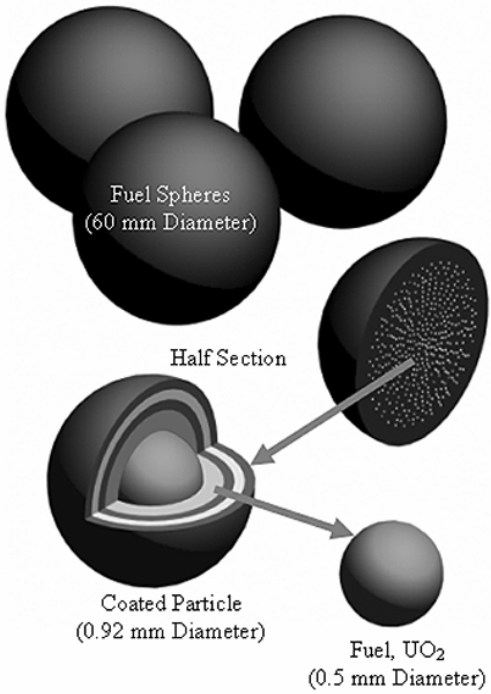
\includegraphics[scale=.5]{pics/triso1.png}
  \caption[Ilustrasi bentuk bahan bakar \textit{pebble}]{Ilustrasi bentuk bahan bakar \textit{pebble} \cite{wang2004integrated}}
  \label{fig:bentukpebble}
\end{figure} 

Bahan bakar berjenis \textit{pebble} ini memiliki komponen utama yang dalam Gambar \ref{fig:bentukpebble} disebut sebagai \textit{coated particle}. Komposisi elemen pelapis (\textit{coated}) dapat diilustrasikan dalam Gambar \ref{fig:pelapis}. Dalam upaya menguasai teknologi reaktor berjenis HTGR melalui pengembangan RDE, salah tugas yang harus dilaksanakan adalah penguasaan analisis kegagalan bahan bakarnya, khususnya ketika terjadi kecelakaan.

Beragam model analisis telah dikembangkan, salah satunya yang dikembangkan oleh Wang \cite{wang2004integrated}. Selain itu, terdapat sebuah model sederhana yang dikembangkan oleh Verfondern dalam PANAMA \cite{VERFONDERN201484}. Pada model tersebut, bahan bakar disebut gagal jika kekuatan lapisan SiC (\textit{Silicon Carbide}) lebih kecil daripada tekanan internal dari lapisan di bawahnya (perhatikan Gambar \ref{fig:pelapis}). Model inilah yang akan diterapkan dalam TRIAC (\textit{TRIso Analysis Code}).

\begin{figure}[h]
  \centering
  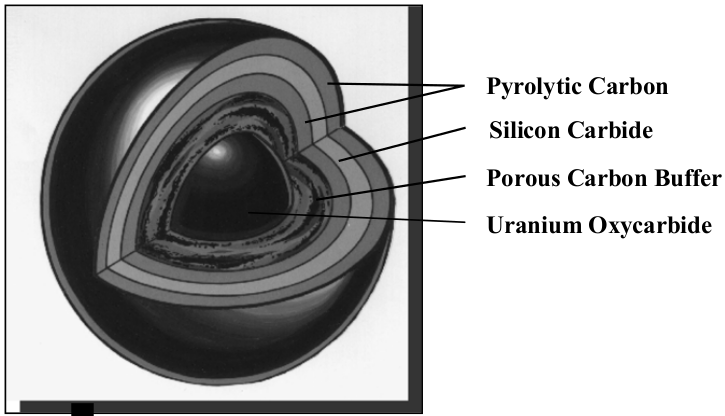
\includegraphics[scale=.5]{pics/triso.png}
  \caption[Komposisi elemen pelapis partikel]{Komposisi elemen pelapis partikel \cite{wang2004integrated}}
  \label{fig:pelapis}
\end{figure}

\chapter{Alur Perhitungan}
\section{Pendahuluan}
Secara umum, perhitungan TRIAC mengikuti diagram alir seperti pada Gambar \ref{fig:flowchart} berikut. Sementara kode sumbernya disajikan dalam Listing \ref{triac.py} yang dibangun sepenuhnya berbasis pengetahuan yang diperoleh dari dokumen laporan teknis \cite{report1}.
\begin{figure}[h]
  \centering
  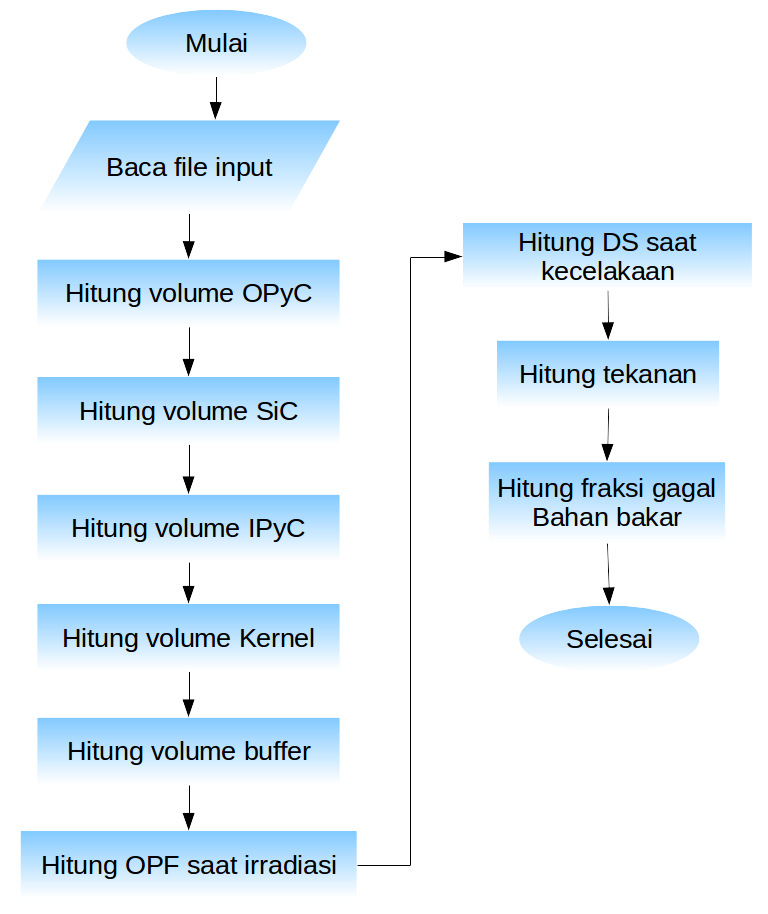
\includegraphics[scale=.5]{pics/Flowchart.png}
  \caption{Diagram alir perhitungan TRAIC}
  \label{fig:flowchart}
\end{figure}

\vfill
\scriptsize
\lstinputlisting[language=python, numbers=left, numberstyle=\tiny, caption=triac.py, showstringspaces=false, label=triac.py]{../TRIAC/inputdata.py}
\normalsize

\section{Membaca \textit{file input}}
Sub rutin ini ditujukan untuk membaca file input dengan format seperti terdapat pada Lampiran 1. Sub rutin ini menggunakan skema yang kaku karena identifikasi nilai-nilai yang akan dibaca ditentukan oleh suatu teks tertentu. Setelah teks yang menjadi penanda, nilai-nilai yang dibutuhkan dibaca. Tetapi, nilai tersebut dapat langsung berada dalam satu baris bersama dengan teks penanda, atau berada pada baris yang berbeda. Sub rutin ini terdapat pada baris ke-3 s/d baris ke-69 dalam Listing \ref{triac.py}

Terdapat empat jenis data yang perlu dibaca dari \textit{file input} dalam Lampiran 1, masing-masing adalah sebagai berikut.
\begin{enumerate}
  \item Data tentang geometri \textit{pebble}. Data ini diidentifikasi menggunakan teks yang didefinisikan oleh variabel \texttt{statusGeometry} (baris ke-5 pada Listing \ref{triac.py}). Di dalam data geometri, terdapat empat data berbeda, masing-masing secara berurutan adalah panjang jejari \textit{pebble} terluar, OPyC (\textit{Outer Pyrolitic Carbon}), SiC (\textit{Silicon Carbide}), IPyC (\textit{Inner Pyrolitic Carbon}), \textit{buffer} dan kernel. Data geometri akan digunakan untuk menghitung volume setiap elemen pelapis (Gambar \ref{fig:pelapis}). Yang perlu diperhatikan adalah data jari-jari yang disajikan adalah jarak dari pusat bahan bakar sampai titik terluar dari setiap lapisan. Karena itu, volume suatu lapisan harus mempertimbangkan lapisan-lapisan di dalamnya. Data geometri disimpan dalam variabel diberi nama \texttt{dimensi} dan dalam bentuk \texttt{list} (baris ke-10 dalam Listing \ref{triac.py}).
  \item Data tentang kekuatan SiC. Data ini diidentifikasi menggunakan teks yang didefinisikan oleh variabel \texttt{statusCharacteristics} (baris ke-6 pada Listing \ref{triac.py}). Ada empat nilai yang perlu dibaca terkait kekuatan SiC, masing-masing adalah SiC \textit{Tensile Strength} [Pa],	\textit{Weibull Modulus	Burnup} [FIMA],	\textit{Fission Yield of stable fission gasses} [Ff],	\textit{Fast Neutron Fluence}	dan rasio berat Th terhadap U-235 pada kernel. Data terkait kekuatan SiC disimpan dalam variabel yang diberi nama \texttt{characteristics} dalam bentuk \texttt{list} (baris ke-11 dalam Listing \ref{triac.py}).
    \item Data tentang sejarah irradiasi. Data ini diidentifikasi menggunakan teks yang didefinisikan oleh variabel \texttt{statusIrradiation} (baris ke-7 pada Listing \ref{triac.py}). Data ini merupakan data temperatur bahan bakar \textit{pebble} pada selang waktu tertentu. Sebagai contoh, data yang disajikan pada Lampiran 1 diambil pada selang waktu 17 hari. Data sejarah irradiasi disimpan dalam variabel yang diberi nama \texttt{irradiation} dalam bentuk \texttt{list}. Setiap elemen adalah \texttt{list} yang secara \textit{nested} terdiri dari dua elemen yang mewakili data kolom kedua dan ketiga tiap akuisisi (baris ke-12 pada Listing \ref{triac.py}). Ilustrasinya adalah seperti $[[0,	593], [17,	833], \ldots]$. Data tentang nomor urut tidak digunakan karena selain tidak diperlukan dalam perhitungan, akan menyulitkan proses interpolasi yang akan diterapkan berikutnya.
    \item Data tentang sejarah kecelakaan. Data ini diidentifikasi menggunakan teks yang didefinisikan oleh variabel \texttt{statusAccident} (baris ke-8 pada Listing \ref{triac.py}). Data ini memiliki pola yang sama dengan data sejarah irradiasi. Data sejarah keselakaan disimpan dengan cara yang sama seperti data tentang sejarah irradiasi tetapi dengan nama \texttt{accident} (baris ke-13 pada Listing \ref{triac.py}). Ilustrasinya adalah seperti $[[0,	1033], [0.0271,	1033],\ldots]$
\end{enumerate}.
 
\section{Menghitung OPF saat irradiasi}
\label{sec:OPF}
OPF (\textit{Oxygen Per Fission}) adalah jumlah atom oksigen yang terlepas selama fisi atom $U^{235}$ atau $Pu^{239}$. Atom oksigen ini mempengaruhi terbentunya senyawa CO yang akan meningkatkan tekanan internal dalam bahan bakar. Pembentukan senyawa CO juga dipengaruhi oleh temperatur, waktu serta jenis partikel kernel. 

Nilai OPF didekati oleh persamaan (\ref{eq:opf1}). Nilai $n$ dalam persamaan (\ref{eq:opf1}) sama dengan banyaknya data sejarah irradiasi. Nilai $\Delta_{i}$ merupakan selisih waktu dari sejarah irradiasi yang dicatat. Nilainya akan berubah dengan berubahnya rentang pencatatan temperatur irradiasi. Jika dalam contoh kasus yang disajikan pada Lampiran 1, rentang waktu pencatatan temperatur irradiasi dilakukan setiap $17$ hari, maka $\Delta_{i}$ adalah $17$ hari atau $17 x 24 x 3600$ detik. $t_B$ adalah waktu irradiasi total bahan bakar, sedangkan $\overline{t_i}$ waktu irradiasi ketika pencatatan dilakukan.

\begin{equation}
  OPF \simeq \sum_{i=1}^{n} g(\overline{t_{i}}) \cdot (t_{B}-\overline{t_{i}}) \cdot \Delta t_{i}
  \label{eq:opf1}
\end{equation}
 
Tetapi, nilai OPF juga didefinisikan seperti persamaan (\ref{eq:opf2}), dengan nilai $g(\overline{t_{i}})$ didefinisikan oleh persamaan (\ref{eq:gt}). Nilai $R$ pada persamaan (\ref{eq:gt}) adalah konstanta gas sebesar $8.3143 [\frac{J}{mole \cdot K}]$.
\begin{equation}
  OPF = \frac{g(T)}{2} \cdot t^2
  \label{eq:opf2}
\end{equation} 
 
\begin{equation}
  \frac{g(T)}{2}=8.32 \cdot 10^{-11} \cdot e^{\frac{-163000}{R \cdot T}}
  \label{eq:gt}
\end{equation} 
 
Nilai OPF selanjutnya digunakan untuk menghitung nilai temperatur irradiasi ($T_B$) dari persamaan (\ref{eq:TB}). Formula empiris tersebut sesuai untuk jenis bahan bakar $UO_2$.
\begin{equation}
  \log OPF=-10.08-\frac{0.85 \cdot 10^4}{T_B} + 2 \cdot \log t_B
  \label{eq:TB}
\end{equation} 

Sedangkan nilai $T_B$ akan digunakan untuk menghitung $DS$, faktor berkurangnya koefisien difusi ($s^{-1}$) dari gas hasil fisi di dalam partikel kernel. Nilainya untuk bahan bakar $UO_2$ memenuhi persamaan (\ref{eq:DS}).

\begin{equation}
  \log DS=-2.30-\frac{0.8116 \cdot 10^4}{T_B}
  \label{eq:DS}.
\end{equation}

Terakhir, $DS$ akan digunakan untuk menghitung sebuah nilai tak berdimensi $\tau_i$ yang memenuhi persamaan (\ref{eq:taui}).
\begin{equation}
  \tau_i=DS(T_B) \cdot t_B
  \label{eq:taui}
\end{equation}

\section{Menghitung DS saat kecelakaan}
Seperti telah dijelaskan dalam sub bab \ref{sec:OPF}, $DS$ adalah faktor berkurangnya koefisien difusi gas hasil fisi dalam partikel kernel. Sekarang, faktor ini dihitung ketika kondisi kecelakaan terjadi. Kita memerlukan sejarah temperatur bahan bakar setelah kecelakaan terjadi serta $\tau_i$. yang telah dihitung di persamaan (\ref{eq:taui}).

Dengan menggunakan persamaan (\ref{eq:taui}), kita dapat menghitung nilai $DS$ dengan temperatur kecelakaan yang tercatat.  Kemudian, kita perlu menghitung nilai $\tau_A$ dengan persamaan (\ref{eq:taui}) tetapi dengan nilai temperatur dan waktu setelah terjadi kecelakaan. Selanjutnya, dengan modal nilai $\tau_i$ dan $\tau_A$ kita akan menghitung nilai $Fd$, yang merupakan faktor fisi gas Xe dan Kr (yang dominan). Nilai $Fd$ dihitung dengan persamaan (\ref{eq:Fd}).
\begin{equation}
  Fd=\frac{(\tau_i + \tau_A) \cdot f(\tau_i + \tau_A) - \tau_A \cdot f(\tau_A)}{\tau_i}
  \label{eq:Fd}
\end{equation}

Sedangkan nilai $f(\tau)$ dihitung menggunakan persaamaan (\ref{eq:ftau}). Batas atas nilai $n$ pada persaamaan (\ref{eq:ftau}) dapat menggunakan nilai yang cukup besar, misalnya $1000$, atau ketika dua nilai berdekatan yang dihasilkan hanya berselisih kurang dari $10^{-20}$. Idealnya, suku penjumlahan sebanyak $n$ akan semakin baik jika hasilnya mendekati $1$.
\begin{equation}
  f(\tau)=1-\frac{6}{\tau} \cdot \sum_{n=1}^{\infty} \left( \frac{1-e^{-n^2 \cdot \pi^2 \cdot \tau}}{n^4 \cdot \pi^4} \right)
  \label{eq:ftau}
\end{equation}

%Di level implementasi, perhitungan $DS$ saat kecelakaan didistribusi ke dalam beberapa fungsi seperti terlihat pada Listing \ref{triac.py}. Masing-masing fungsi tersebut adalah \texttt{DS(accident,tauI)} dan \texttt{FD(tauA,tauI)}.

\section{Menghitung tekanan}
Tekanan adalah variabel yang penting dalam tahapan analisis ini karena akan menentukan fraksi gagal bahan bakar. Untuk menghitung tekanan yang timbul ketika kecelakaan terjadi pada waktu tertentu, sehingga menyebabkan panas tertentu, digunakan persamaan (\ref{eq:tekanan}) \cite{wang2004integrated}. 
\begin{equation}
  p=\frac{(F_d \cdot F_f + OPF) \cdot F_b \cdot (\frac{V_f}{V_k}) \cdot R \cdot T}{ V_m}
  \label{eq:tekanan}
\end{equation}
dengan :
\begin{description}
  \item $F_d$ = fraksi relatif gas fisi yang lepas 
  \item $F_f$ = produk fisi yang dihasilkan dari gas fisi stabil, $F_f$=0.31
  \item OPF = jumlah atom oksigen setiap terjadi fisi saat terjadi kecelakaan
  \item $F_b$ = \textit{burnup} logam berat (FIMA)
  \item $V_f$ = fraksi void [$m^3$], terkait dengan $50\%$ volume buffer 
  \item $V_k$ = volume kernel [$m^3$]
  \item $V_m$ = volume molar dalam partiekl kernel $\left[\frac{m^3}{mole} \right]$
  \item $R$ = konstanta gas, 8.3143 $\left[\frac{J}{(mole \cdot K)} \right]$
\end{description}

Khusus untuk variabel $OPF$, karena perhitungan tekanan dilakukan ketika terjadi kecelakaan, digunakanlah persamaan (\ref{eq:opf3}). Persamaan (\ref{eq:opf3}) mirip dengan persamaan (\ref{eq:TB}) dengan penambahan suku ke-3.
\begin{equation}
  \log OPF=-10.08-\frac{0.85 \cdot 10^4}{T_B} + 2 \cdot \log t_B - 0.04 \cdot \left( \frac{10^4}{T} + \frac{10^4}{T_B + 75} \right)
  \label{eq:opf3}
\end{equation}

\section{Fraksi gagal bahan bakar}
Tahapan terkahir dari analisis ini adalah perhitungan fraksi gagal bahan bakar. Secara umum, fraksi gagal bahan bakar dipengaruhi sejumlah sebab. Dalam analisis yang dilakukan TRAIC (dan juga PANAMA sebagai acuannya), gagalnya bahan bakar dapat disebabkan oleh 3 sebab. Ketiganya adalah sebagai berikut.
\begin{enumerate}
\item Pabrikasi ($\phi_0$). Dalam analisis ini, nilai $\phi_0$ diasumsikan sama dengan $0$.
\item Berkurangnya \textit{tensile strength} lapisan SiC ($\phi_1$). Hal ini dapat terjadi karena
\begin{itemize}
\item proses irradiasi maupun
\item meningkatnya temperatur secara signifikan ketika terjadi kecelakaan) atau disebut juga \textit{grain boundary}.
\end{itemize}  
\item Dekomposisi termal pada temperatur tinggi yang menyebabkan terjadinya \textit{weight loss} pada lapisan SiC ($\phi_2$).
\end{enumerate}

Ketiga sebab terjadinya kegagalan bahan bakar tersebut mengikuti persamaan (\ref{eq:gagal1}).
\begin{equation}
  \phi_{total}=1-(1-\phi_1) -(1-\phi_2)
  \label{eq:gagal1}
\end{equation}

\subsection{Fraksi gagal akibat berkurangnya \textit{tensile strength}}
Nilai fraksi gagal bahan bakar pada waktu $t$ setelah terjadinya kecelakaan diperoleh dengan persamaan (\ref{eq:gagal}).
\begin{equation}
  \phi_1(t,T)=1-e^{-\ln 2 \cdot \left(\frac{\sigma_t}{\sigma_o}\right)^m}
  \label{eq:gagal}
\end{equation}
dengan :
\begin{description}
  \item $\sigma_o$=\textit{tensile strength} dari SiC [Pa] pada akhir irradiasi
  \item $\sigma_t$=tekanan yang dialami SiC [Pa] akibat tekanan gas internal
\end{description}

Variabel tekanan internal pada SiC ($\sigma_t$) dihitung dengan dengan persamaan (\ref{eq:sigmaT}). Pada persamaan (\ref{eq:sigmaT}), jari-jari lapisan SiC merupakan rerata karena lapisan SiC memang memiliki ketebalan yang nilai awalnya diwakili oleh variabel $d_o$.
\begin{equation}
  \sigma_t =\frac{r \cdot p}{2 \cdot d_o} \cdot \left( 1+\frac{\dot{v} \cdot t}{d_o} \right)
  \label{eq:sigmaT}
\end{equation}
dengan :
\begin{description}
  \item $r$=rerata jari-jari SiC, $\left( 0.5 \cdot \left( r_a^3 + r_i^3 \right)\right)^{\frac{1}{3}}$ [m]
  \item $d_o$=ketebalan awal lapisan SiC, $r_a - r_i$ [m]
  \item $p$=tekanan gas fisi dalam partikel [Pa]
  \item $\dot{v}$=laju korosi sebagai fungsi temperatur (T), $\left[\frac{m}{s}\right]$
\end{description}

Sedangkan variabel laju korosi ($\dot{v}$) dihitung dengan persamaan (\ref{eq:korosi}), mirip dengan persamaan (\ref{eq:gt}) dengan perbedaan pada konstanta.
\begin{equation}
  \dot{v}=5.87 \cdot 10^{-7} \cdot e^{-\left( \frac{179500}{R \cdot T}\right)}
  \label{eq:korosi}
\end{equation}

Selanjutnya, variabel \textit{tensile strength} lapisan SiC, penurunan nilainya mengikuti persamaan (\ref{eq:strengthSiC}). Variabel $\sigma_{oo}$ merupakan \textit{tensile strength} awal sebelum diiradiasi. Nilainya merupakan sesuatu yang dapat diukur. Sedangkan $\Gamma$ dan $\Gamma_s$ masing-masing merupakan \textit{fluence} netron cepat $\left[ 10^{25}m^{-2} EDN\right]$ dan \textit{fluence} yang dipengaruhi temperatur irradiasi. Nilai $\Gamma_s$ ditentukan menggunakan persamaan (\ref{eq:fluenceS}). Nilai minimum $\sigma_{oo}$ merupakan nilai awal \textit{tensile strength} dan diasumsikan sama dengan 196 [MPa]. Tentunya, dengan perlakuan irradiasi yang sama, lapisan SiC dengan nilai awal \textit{tensile strength} terkecil akan memiliki nilai akhir \textit{tensile strength} yang juga kecil.
\begin{equation}
  \sigma_o = \sigma_{oo} \cdot \left( 1- \frac{\Gamma}{\Gamma_s} \right)
  \label{eq:strengthSiC}
\end{equation}

\begin{equation}
  \log \Gamma_s = 0.556 + \frac{0.065 \cdot 10^4}{T_B}
  \label{eq:fluenceS}
\end{equation}

\textit{Tensile strength} lapisan SiC yang dihitung menggunakan persamaan (\ref{eq:strengthSiC}) merupakan nilai yang berlaku pada satu \textit{coated particle}. Padahal, ada sangat banyak \textit{coated particle} yang dioperasikan. Karena itu, diperlukan perhitungan yang mempertimbangkan variabel ini untuk semua distribusi \textit{coated particles}. Dengan pendekatan yang sama seperti persamaan (\ref{eq:strengthSiC}), persamaan (\ref{eq:strengthSiCdist}) dibangun.

\begin{equation}
  m_o = m_{oo} \cdot \left( 1- \frac{\Gamma}{\Gamma_m} \right)
  \label{eq:strengthSiCdist}
\end{equation}
dengan $\log \Gamma_m = 0.394 + \frac{0.065 \cdot 10^4}{T_B}$ dan nilai $m_{oo}=2$ sebagai nilai terkecilnya. Nilai $m_o$ pada persamaan (\ref{eq:strengthSiCdist}) kemudian akan disubstitusi ke persamaan (\ref{eq:gagal}) sebagai $m$.


Selain korosi karena proses irradiasi, lapisan SiC juga dapat terkorosi karena \textit{grain Boundary}. Jika korosi akibat irradiasi tergantung pada sejarah irradiasi yang dialami bahan bakar dan terjadi sebelum kecelakaan, maka korosi karena \textit{grain Boundary} terjadi setelah kecelakaan. Penurunan nilai distribusi \textit{tensile strength} akibat meningkatnya temperatur karena kecelakaan mengikuti persamaan (\ref{eq:grainBoundary}).
\begin{equation}
  m=m_o \cdot \left( 0.44 + 0.56 \cdot e^{-\dot{\eta} \cdot t}\right)
  \label{eq:grainBoundary}
\end{equation}

di mana nilai $\dot{\eta}$ mengikuti persamaan {\ref{eq:eta}} dengan pola yang sama seperti persamaan (\ref{eq:korosi}).
\begin{equation}
  \dot{\eta}=0.565 \cdot e^{\left(\frac{-187400}{R \cdot T}\right)} [s^{-1}]
  \label{eq:eta}
\end{equation}

\subsection{Fraksi gagal bahan bakar akibat \textit{weight loss}}
Laju \textit{weight loss} yang terjadi akibat tingginya temperatur saat terjadi kecelakaan mengikuti persamaan (\ref{eq:weightLoss}).
\begin{equation}
  k=k_o \cdot e^{\frac{-Q}{R \cdot T}}
  \label{eq:weightLoss}
\end{equation}
dengan $Q=556 \left[ \frac{kJ}{mol}\right]$ dan $k_o$ adalah faktor frekuensi yang tergantung pada jenis partikel.

Selanjutnya, diasumsikan bahwa partikel TRISO tergantung pada apa yang disebut sebagai ''\textit{action integral}'', dan disimbolkan dengan $\zeta$ yang nilainya mengikuti persamaan (\ref{eq:zeta}).
\begin{equation}
  \zeta=\int_{t_1}^{t_2} k(T) dt
  \label{eq:zeta}
\end{equation}
dengan $K(T)$ adalah nilai yang menggambarkan sejarah kondisi partikel yang bergantung pada temperatur dan waktu.

Secara numerik, persamaan (\ref{eq:zeta}) dapat dituliskan sebagai persamaa (\ref{eq:zeta1}).
\begin{equation}
  \zeta(t_2)=\zeta(t_1)+k(T_m) \cdot (t_2 - t_1)
  \label{eq:zeta1}
\end{equation}
dengan $k(T_m)=\frac{375}{d_o} \cdot e^{\left(\frac{-556000}{R \cdot T_m}\right)}$.

Kemudian, fraksi gagal $\phi_2$ sedemikian rupa sehingga nilainya $\leq 1$. Karena itu, variabel $\phi_2$ selanjutnya didefinisikan sebagai persamaan (\ref{eq:phi2}).
\begin{equation}
\phi_2(t,T)=1-e^{-\alpha \cdot \zeta^{\beta}}
\label{eq:phi2}
\end{equation}

Nilai $\alpha$ dan $\beta$ kemudian ditentukan secara empiris. Dan berdasarkan penelitian empiris sebelumnya terhadap partikel $UO_2$, diperoleh nilai $\alpha=\ln 2=0.693$, sedangkan nilai $\beta=0.88$.

Dalam TRIAC, faktor fraksi gagal ini tidak akan dipertimbangkan. Hal ini disebabkan karena kondisi ini terjadi pada temperatur di atas $2000\,^{\circ}{\rm C}$. Sementara RDE tidak dirancang untuk sampai pada temperatur tersebut.

% Daftar Pustaka
\bibliographystyle{IEEEtran}
\bibliography{report}

\begin{appendix}
	%
% @author  Andreas Febrian
% @version 1.00 
% 
% Hanya sebuah pembatas bertuliskan LAMPIRAN ditengah halaman. 
% 

\begin{titlepage}
	\centering 
	\vspace*{6cm}
	\noindent \Huge{LAMPIRAN}
	\addChapter{LAMPIRAN}
\end{titlepage}

	\setcounter{page}{2}
	%-----------------------------------------------------------------------------%
\addChapter{Lampiran 1}
\chapter*{Lampiran 1: Contoh file input}
\label{lamp:inputExample}
%-----------------------------------------------------------------------------%
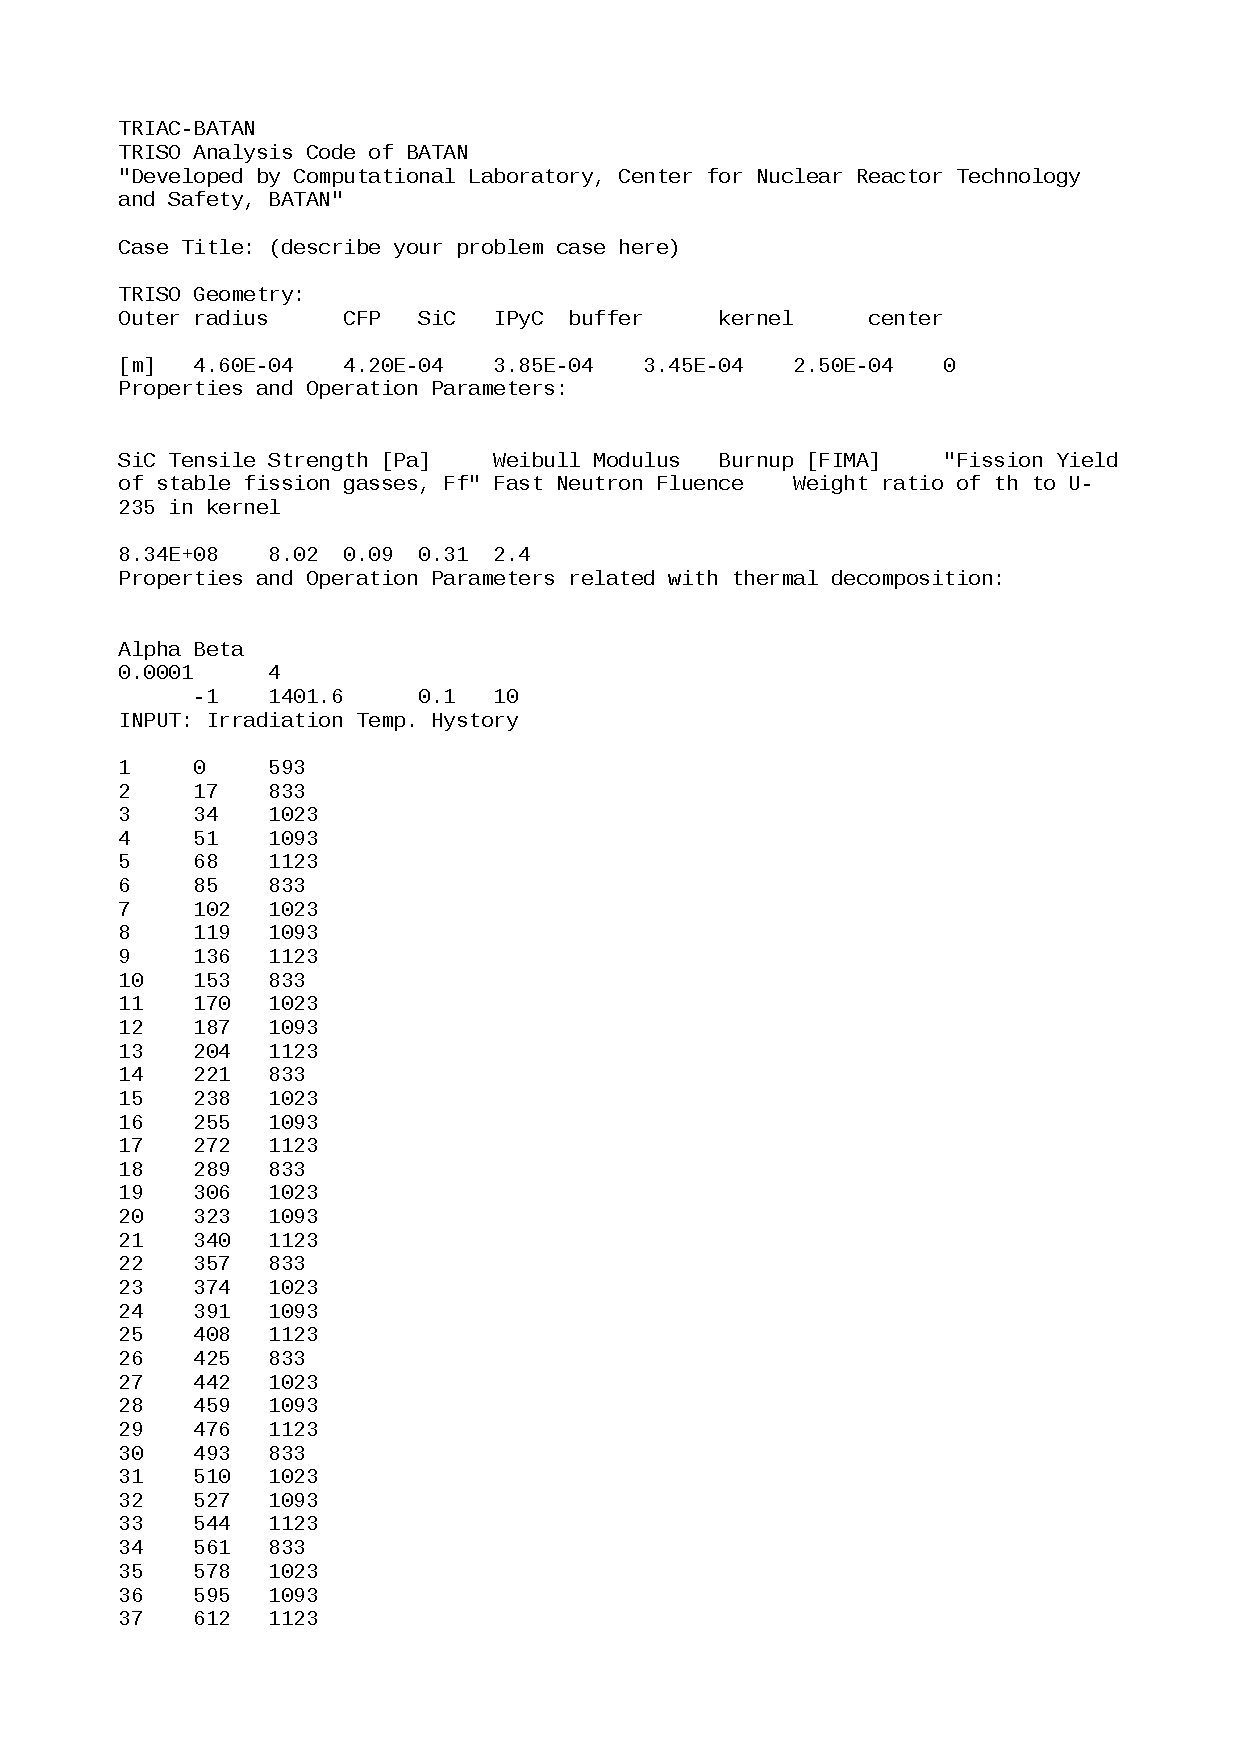
\includepdf[pages={1-}]{inputExample.pdf}
%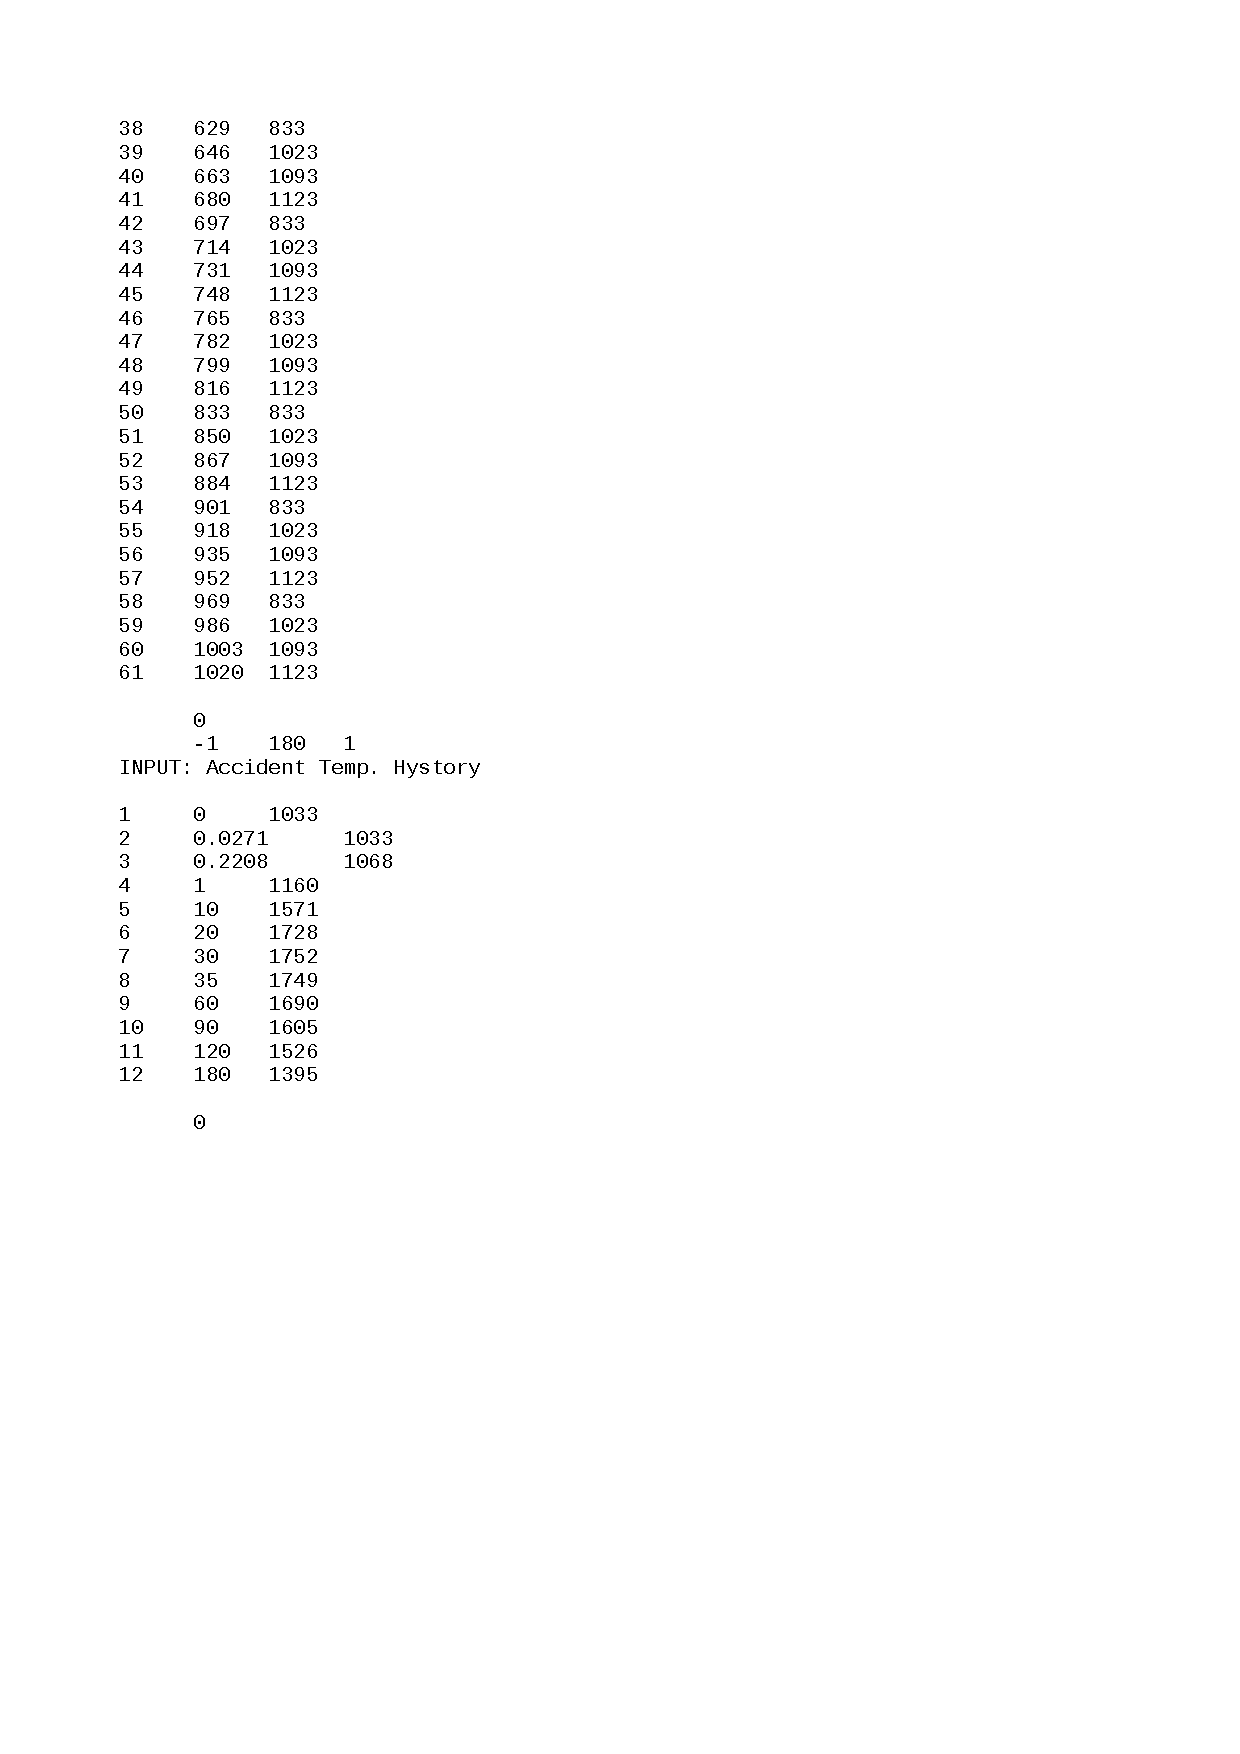
\includepdf{inputExample2}

\addChapter{Lampiran 2: InputData.py}
\chapter*{Lampiran 2: InputData.py}
\scriptsize
\lstinputlisting[language=python, numbers=left, numberstyle=\tiny, caption=InputData.py, showstringspaces=false, label=InputData.py]{../Uji/InputData.py}
\normalsize

\addChapter{Lampiran 3: interpolasi.py}
\chapter*{Lampiran 3: interpolasi.py}
\scriptsize
\lstinputlisting[language=python, numbers=left, numberstyle=\tiny, caption=Interpolasi.py, showstringspaces=false, label=Interpolasi.py]{../TRIAC/Interpolasi.py}
\normalsize

\addChapter{Lampiran 4: core.py}
\chapter*{Lampiran 4: core.py}
\scriptsize
\lstinputlisting[language=python, numbers=left, numberstyle=\tiny, caption=core.py, showstringspaces=false, label=core.py]{../Uji/core.py}
\normalsize

\addChapter{Lampiran 5: triac.py}
\chapter*{Lampiran 5: triac.py}
\scriptsize
\lstinputlisting[language=python, numbers=left, numberstyle=\tiny, caption=triac.py, showstringspaces=false, label=triac.py]{../Uji/triacc.py}
\normalsize

\end{appendix}

\end{document}
